%
% Niniejszy plik stanowi przykład formatowania pracy magisterskiej na
% Wydziale MIM UW.  Szkielet użytych poleceń można wykorzystywać do
% woli, np. formatujac wlasna prace.
%
% Zawartosc merytoryczna stanowi oryginalnosiagniecie
% naukowosciowe Marcina Wolinskiego.  Wszelkie prawa zastrzeżone.
%
% Copyright (c) 2001 by Marcin Woliński <M.Wolinski@gust.org.pl>
% Poprawki spowodowane zmianami przepisów - Marcin Szczuka, 1.10.2004
% Poprawki spowodowane zmianami przepisow i ujednolicenie 
% - Seweryn Karłowicz, 05.05.2006
% Dodanie wielu autorów i tłumaczenia na angielski - Kuba Pochrybniak, 29.11.2016

% dodaj opcję [licencjacka] dla pracy licencjackiej
% dodaj opcję [en] dla wersji angielskiej (mogą być obie: [licencjacka,en])
\documentclass[licencjacka,en]{pracamgr}

\usepackage{graphicx} %package to manage images
\graphicspath{ {./images/} }

\usepackage[rightcaption]{sidecap}

\usepackage{wrapfig}

% Dane magistranta:
% \autor{Adam Deryło, Adrian Hess, Magdalena Pałkus, Michał Skwarek}{34234234}

% Dane magistrantów:
\autor{Adam Deryło}{432952}
\autori{Adrian Hess}{431481}
\autorii{Magdalena Pałkus}{421537}
\autoriii{Michał Skwarek}{418426}
%\autoriv{Autor nr Cztery}{432145}
%\autorv{Autor nr Pięć}{342011}

\title{GPU acceleration of CCSDS Rice decoding}
\titlepl{Akcerleracja GPU dekodowania CCSDS Rice}

%\tytulang{An implementation of a difference blabalizer based on the theory of $\sigma$ -- $\rho$ phetors}

%kierunek: 
% - matematyka, informacyka, ...
% - Mathematics, Computer Science, ...
\kierunek{Computer Science}

% informatyka - nie okreslamy zakresu (opcja zakomentowana)
% matematyka - zakres moze pozostac nieokreslony,
% a jesli ma byc okreslony dla pracy mgr,
% to przyjmuje jedna z wartosci:
% {metod matematycznych w finansach}
% {metod matematycznych w ubezpieczeniach}
% {matematyki stosowanej}
% {nauczania matematyki}
% Dla pracy licencjackiej mamy natomiast
% mozliwosc wpisania takiej wartosci zakresu:
% {Jednoczesnych Studiow Ekonomiczno--Matematycznych}

% \zakres{Tu wpisac, jesli trzeba, jedna z opcji podanych wyzej}

% Praca wykonana pod kierunkiem:
% (podać tytuł/stopień imię i nazwisko opiekuna
% Instytut
% ew. Wydział ew. Uczelnia (jeżeli nie MIM UW))
\opiekun{Paweł Gora\\
  Faculty of Mathematics, Informatics and Mechanics, University of Warsaw\\
  }

% miesiąc i~rok:
\date{Jan 2023}

%Podać dziedzinę wg klasyfikacji Socrates-Erasmus:
\dziedzina{ 
%11.0 Matematyka, Informatyka:\\ 
%11.1 Matematyka\\ 
% 11.2 Statystyka\\ 
11.3 Informatics, Computer Science \\ 
%11.3 Informatyka\\ 
%11.4 Sztuczna inteligencja\\ 
%11.5 Nauki aktuarialne\\
%11.9 Inne nauki matematyczne i informatyczne
}

%Klasyfikacja tematyczna wedlug AMS (matematyka) lub ACM (informatyka)
\klasyfikacja{D. Software\\
  D.1.3. Concurrent Programming\\
  I.4.2. Compression (Coding) \\ }

% Słowa kluczowe:
\keywords{CCSDS Rice coding, GPU, Compute Unified Device Architecture (CUDA)}

% Tu jest dobre miejsce na Twoje własne makra i~środowiska:
\newtheorem{defi}{Definicja}[section]

% koniec definicji

\begin{document}
\maketitle

%tu idzie streszczenie na strone poczatkowa
\begin{abstract}
	TBD
\end{abstract}

\tableofcontents
%\listoffigures
%\listoftables

\chapter{Introduction}
\section{Background and motivation}
Machine learning (ML) has rapidly become a crucial tool for solving complex problems in a variety of domains, including computer vision, natural language processing, and speech recognition. However, ML pipelines can often experience significant bottlenecks due to multi-stage data processing pipelines that include loading, decoding, cropping, resizing, and other augmentations. This is particularly true when these processing steps are executed on a CPU, which is frequently the case. Since, most of the machine learning training is already GPU accelerated due to ML workloads having a highly parallel nature, it is a natural progression to solve data processing bottlenecks by harnessing GPU acceleration.

One such bottleneck is decompression of RICE coded data, which is one of the most commonly used compression algorithms used in astronomy and astrophysics. Currently, there are only CPU-based solutions for decoding RICE compressed data. This, substantially hinders application of machine learning solutions in astronomy, especially considering the massive amount of training data already stored in RICE compressed algorithm as well as being produced by observatories all around the world. To illustrate, just Solar Dynamics Observatory (SDO), with limited bandwidth due to being a satellite, is producing 130 megabits of rice coded data per second, that is 500 TB per year.

\section{Problem statement}
The problem at hand is that the current RICE decompression algorithm is a computationally intensive and cannot keep up with the demand for high throughput and real-time processing. The goal of this project is to design and develop a GPU-based RICE decompression algorithm that can significantly accelerate the decompression process and improve the speed, efficiency, and scalability of ML pipelines in astronomy applications.

\section{Research objectives}
The main objectives of this thesis are as follows:

\begin{itemize}
	\item To study the existing literature on GPU acceleration of data compression and RICE decompression.
	\item To analyze the performance of RICE decompression on a CPU and a GPU.
	\item To design and implement a GPU-accelerated RICE decompression algorithm.
	\item To evaluate the performance of the GPU-accelerated RICE decompression algorithm and compare it with the CPU-based RICE decompression algorithm.
	\item And finally, to incorporate findings into NVIDIA Data Loading Library (DALI), so machine learning as well as the astronomy community can utilize our findings.
\end{itemize}

\section{Thesis structure}
In this thesis, we present our attempts at parallelizing the RICE decompression algorithm and CUDA-based implementations of our findings.

Chapter 2 aims to define and explain key terms for our problem space, including the RICE algorithm itself. In the following chapter, we review previous work on the subject. We then present our solution architecture and how it ties into NVIDIA's open-source data loading framework called DALI. Additionally, we introduce the Compute Unified Device Architecture (CUDA) to the reader. In Chapter 5, we propose a parallel implementation of the algorithm on GPU with details. Chapter 6 presents our performance and speedup results. Finally, in Chapter 7, we summarize our findings and conclude the thesis.

\chapter{Key terms}\label{r:pojecia}


\section{RICE}
The RICE algorithm is a well-known, lossless data compression algorithm, that uses a set of variable-length codes to compress data. The essence of this algorithm is using these codes to change symbols that are expected to be more frequent to shorter code words. The algorithm works on data blocks that are encoded independently, it’s not needed to transfer some information between different packets. It improves performance and makes RICE algorithm performance independent of data packet size. The RICE algorithm consists of two main parts: a preprocessor and an adaptive entropy coder.

\section{FITS}
The Flexible Image Transport System (FITS) format is a digital file format that is commonly
utilized in the field of astronomy for storing and transferring scientific data. FITS files
typically contain images, data cubes, and tables of observational data, as well as associated metadata.
One of the key characteristics of FITS is its ability to store multiple data arrays in a single file, which
allows for the efficient storage and transfer of large data sets.
A FITS files are composed of the following FITS structures, in the order listed:
\begin{itemize}
	\item Primary header and data unit (HDU).
	\item Conforming Extensions (optional).
	\item Other special records (optional, restricted).
\end{itemize}
Thus, files usually resemble the following schema:

\centerline{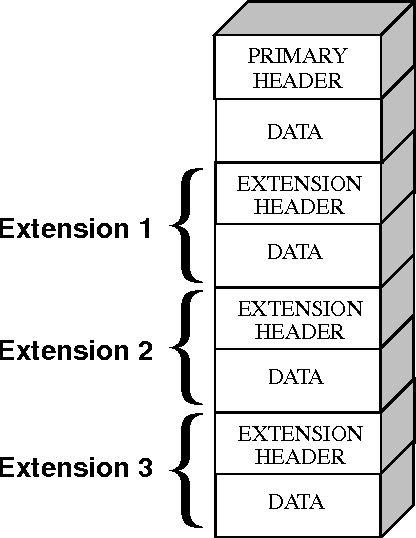
\includegraphics[scale=0.3]{fits}}



Where, all headers, including the primary one, contain relevant metadata as a list of keys and value pairs.
Furthermore, according to the most recent FITS standard published by NASA, there are three types of standard extensions:
\begin{itemize}
	\item IMAGE extensions.
	\item TABLE ASCII-table extensions; and
	\item BINTABLE binary-table extensions
\end{itemize}

\chapter{Previous work}
\section{Rice Coding Suitable for
  GPU Massively Parallel Implementation}
\section{Current decompresssion solutions}

\chapter{Context}\label{r:losers}

\section{NVIDIA}

\section{GPU Programming and CUDA}

\section{DALI}

\chapter{Solution architecture}
\section{DALI readers}
\section{CUDA}

\chapter{GPU acceleration of RICE decoding}
\section{Naive approach}
\section{Optimizing asynchronous data transfer}

\chapter{Results and analysis}
\section{Performance evaluation metrics}
\section{Benchmarking suite}
\section{Comparison of various approaches}

\chapter{Conclusion}
\section{Summary of findings}
\section{Contributions}
\section{Future work}










\begin{thebibliography}{99}
	\addcontentsline{toc}{chapter}{Bibliography}

	\bibitem[Bea65]{beaman} Juliusz Beaman, \textit{Morbidity of the Jolly
		function}, Mathematica Absurdica, 117 (1965) 338--9.


\end{thebibliography}

\end{document}


%%% Local Variables:
%%% mode: latex
%%% TeX-master: t
%%% coding: latin-2
%%% End: